\documentclass[10pt]{article} 
\usepackage[letterpaper, portrait, margin=0.5in]{geometry} 
\usepackage{pbsi}
\usepackage[T1]{fontenc}
\usepackage{graphicx}

\usepackage{hyperref}
\hypersetup{colorlinks=true, linkcolor=blue, filecolor=magenta, urlcolor=cyan}

\begin{document} 
\title{\Huge \bsifamily Notes on OpenCL}
\author{\textit{by Ramkumar Narayanan}}
\date{}
\maketitle 
\tableofcontents
\newpage

% ----------------------------------------------------------------------------------------------------------------
{\color{red} \date{2-Nov-2020}}
\section{Programming Models}
\subsection{Platform Model}
This is a very high level description of the heteregeneous system. 
\begin{enumerate}
	\item \textbf{\textit{Host:}} A device that controls all the OpenCL compatible devices. This is where the main entry point of the program. The host itself could be an OpenCL compatible device.
	\item \textbf{\textit{Compute Devices:}} Each graphics card or the CPU or FPGA's form what is called the compute device. All the compute devies are visible by the host.
	\item \textbf{\textit{Compute Units}} Like the several cores of the processor whether it be a GPU or a CPU. 
	\item \textbf{\textit{Processing Elements:}} Each core will have several small units that does the actual processing call the processing elements.
\end{enumerate}

\begin{figure}[ht]
  \centering
  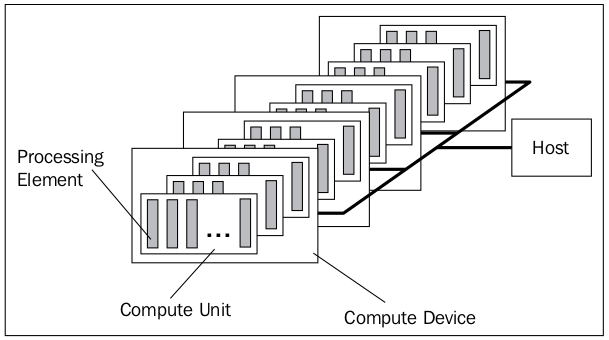
\includegraphics[scale=0.4]{./images/platform_model.png}
  \caption{OpenCL platform model}
  \label{platform_model}
\end{figure}

\subsection{Execution Model}
An OpenCL program has two distinct parts: 1) \textbf{\textit{Host}} program and 2) a collection of one or more \textbf{\textit{kernels}}. Host program runs on the host. Host program is our normal cpp or python code. OpenCL does not define how that is programmed - only how it interacts with the compute device(s).
\begin{enumerate}
	\item \textbf{\textit{OpenCL Kernels:}} Written in C language and compiled with the OpenCL C compiler.
	\item \textbf{\textit{Native Kernels:}} These functions are created outside OpenCL and accesssed within OpenCL through a function pointer.
\end{enumerate}

\subsubsection{Work IDs:}
\textit{\textbf{Work Item:}} Host program issues a command that submits the kernel for execution on the OpenCL device. Each execution of the kernel is called a work item. Each work item running might be running the same sequence of instruction but because of the branching statements and the data selected, its behaviour can differ. 

\textit{\textbf{Index Space:}} When a kernel is submitted by the host program for execution, an index space is created. An instance of kernel is run for each point in the index space.

\textit{\textbf{Work Group:}} Now that we have defined what an index space and work item is, a work group is nothing but an even division of the index space into many blocks of work items as shown in the figure below.

%TODO(ram): Diagram for work items, work groups and index space 

The index space can be 1, 2 or 3 dimensional, they are popularly called the ND space and they span the NDRange. Each work item/group has an ID. They can be global or local. Let us see it with an example. Suppose we have a 2D index space whose size is given by $(G_x, G_y)$; they span values from $0 \rightarrow (G_x-1)$ along the x axis and $0 \rightarrow (G_y-1)$ along the y axis. Suppose, we divide the space into work groups each of size $W_x$ and $W_y$, we have each work group size as $G_x/W_x$ and $G_y/W_y$. A work item can be defined by its global id as $(g_x, g_y)$. Its local ID can be computed by knowing the local work group id the displacement within that work group. 

\subsubsection{Context:}
A context is an OpenCL abstraction for the items required for the setup of running of a program. A \textit{\textbf{host}} defines the kernel, the NDRange, queues that controls the details of how and when the kernels execute. However, the first task on the host is to define the \textit{\textbf{context}} for execution. Context can be defined in the following terms
\begin{enumerate}
	\item \textit{\textbf{Devices:}} A collection of OpenCL devices to be used by the host.
	\item \textit{\textbf{Kernels:}} OpenCL functions that run on the OpenCL devices.
	\item \textit{\textbf{Program Objects:}} The program source code and the executables that implement the kernels. Remember `shaders'? They compile during runtime and create program objects.
	\item \textit{\textbf{Memory Objects:}} Memory visible to OpenCL devices.
\end{enumerate}

Suppose, there are several devices such as a CPU, 2 GPU's etc. A context can be defined by using all the cores of a CPU or either of the GPU's or infact a combination of these. Since OpenCL is heteregeneous hardware compliant, it is not possible to know before hand which device (or combination of devices) the end user is going to run the code on. Hence, the only possibility is to query the resources etc at runtime and build the program object at runtime. Kernel code is either a long string of code within the host program or it can be loaded from a file. Now, with regards to memory, due to several devices, there are several memory spaces to manage. Host has an address space in the CPU and the devices have their own architecture and memeory spaces. To deal with that OpenCL introduces the concept of memory objects. These are explicitely defined on the host and moved between the host and the OpenCL devices.

\vspace{1cm}
{\color{red} \date{13-Nov-2020}}
\subsubsection{Command-Queues:}
The interaction between the host and the device(s) occurs through command queues. The host places the commands into the command queue and then the commands are scheduled for execution in the associated device. OpenCL supports three kinds of commands

\begin{enumerate}
	\item \textit{\textbf{Kernel execution commands:}} Executes a kernel program on the processing elements of the OpenCL device
	\item \textit{\textbf{Memory Commands:}} Transfer data between the host and different memory objects. Host$\rightarrow$Device, Device$\rightarrow$Device.
	\item \textit{\textbf{Synchronization Commands:}} put constraints on the order of execution of the commands.
\end{enumerate}

In a host program, the programmer defines command-queues, memory and program objects, other data structures necessary for execution. The focus shifts to the command-queue. Memory objects are moved from the host to devices, kernel arguments are attached to memory objects. This is then submitted to command-queues for execution. When the kernel has completed its work, the memory object is copied back to the host. Multiple kernels can be submitted and synchronization between then is often required. Finish one before you move onto the next kernel etc can be enforced. Commands in the command queue are executed asynchronously. The host keeps submitting the commands without waiting for the first command to finish. If any synchronization is necessary; that is explicitely done using sync commands. There are two modes of execution

\begin{enumerate}
	\item \textit{\textbf{In order execution:}} commands in the command queue are executed in order after waits.
	\item \textit{\textbf{Out of order exectuion:}} commands in the command queue does not wait for one execution to get over.
\end{enumerate}

By default all versions of OpenCL support inorder exectuion. Out of order execution is necessary for load balancing. For synchronization, commands generate what is called \textit{\textbf{event objects}}. More like a `hey I am done' event. 

One can also have multiple queues within one command queue. The queues run concurrently with no mechanisms for sync between them.

\subsection{Memory Model}
The previous \textit{\textbf{execution model}} described how OpenCL interacts with the host and kernels. In this section we will delve into the different memory objects. OpenCL defines two memory objects \textit{\textbf{buffer objects}} and \textit{\textbf{image objects}}. A buffer object is a contiguous block of memory made available to the kernels. A programmer can map memory chunks to these objects through pointers. An image object on the other hand is specifically restricted to holding images. Sub regions of a buffer object can be assigned as a separate buffer object if need be. 

OpenCL describes five different memory regions viz,

\begin{enumerate}
	\item \textit{\textbf{Global Memory:}} This memory region is visible (read/write access) to all work-items in work-groups. 
	\item \textit{\textbf{Constant Memory:}} Remains constant during the execution of the kernel. All work items have only read-only access to this memory. Host allocates and writes into this chunk of memory.
	\item \textit{\textbf{Local Memory:}} This memory is local to a work-group. All work-items in the work-group can access(r+w) to this memory. Sometimes local memory might be mapped to regions of global memory.
	\item \textit{\textbf{Private Memory:}} This region is private to a work-item and not visible to other work-items.
\end{enumerate}

% TODO(ram): draw the layout of the memory using Ipad

\subsection{Programming Models}

\end{document} 
 
